\documentclass[a4paper]{article}

\usepackage[utf8]{inputenc}
\usepackage[english]{babel}

\usepackage{hyperref}
\usepackage{graphicx}
\usepackage[parfill]{parskip}
\usepackage{minted}

\graphicspath{ {./img/} }

\begin{document}

\title{The Octa.Space project white paper}

\author{Octa.Space\\development team}

\maketitle

\begin{abstract}
Octa.Space project aims to provide the functional and transparent way to
perform computiations in distributed environment, storing/serving any amounts of data and so on.

The nature of the computiations may vary from machine learning to any other computiations which requires massive compuation power.

In this document we explain how and which methods and technologies are used to implement the project.

\end{abstract}

\section{Introduction}

A distributed system is a collection of autonomous computing elements
that appears to its users as a single coherent system\cite{distributedsystems}

\section{Computation units}

Compuation units aka octa-nodes is a primary component in the Octa.Space infrastructure.
They are responsible for providing the compuation power for solving the tasks.
In general the octa-node is a computer with some amount of CPUs, GPUs, memory and disk space.
Each node can be used for computation or/and data storing and serving.
\\

To start accepting and solving tasks the special software must be installed on the computer.
This software is called \textbf{ORC} it's acts as middleware between OS and compuation environments.
\\

\textbf{ORC} is responsible for the following:

\begin{itemize}
    \item Exposing secure RPC channel to receive commands
    \item Organizing isolated environments for tasks
    \item Collecting the system parameters, metrics and loads
    \item Providing data storage interface
    \item Self-upgrade and self-maintenance operations
\end{itemize}

\begin{figure}[h]
\centering
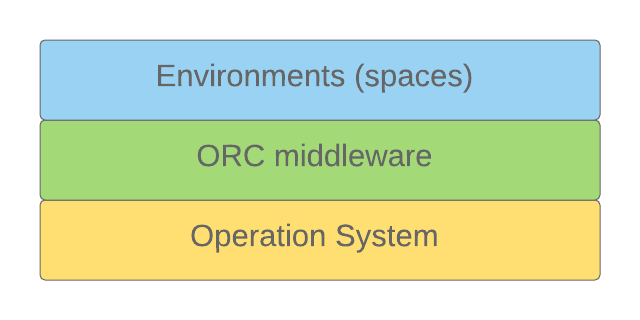
\includegraphics[width=5cm]{os-orc-spaces}
\caption{Octa-node layers}
\end{figure}

Secure channel is implemented using HTTPS\cite{https} protocol with validating each request using security token.

Security token is a fingerprint of the node, it's calculated in the following manner:

\begin{verbatim}
    Token = SHA256(IP, Timestamp, RandomInt)
\end{verbatim}

Where

\begin{itemize}
    \item IP - node public IPv4 address
    \item Timestamp - the time when node is installed in milliseconds
    \item RandomInt - random integer number
\end{itemize}

Commands recieved by the node is executed in the isolated environments.
These environments called \textbf{spaces} and implemented using Docker technology.

\textbf{Spaces} divided into two types: mandatory and task specific

\begin{figure}[h]
\centering
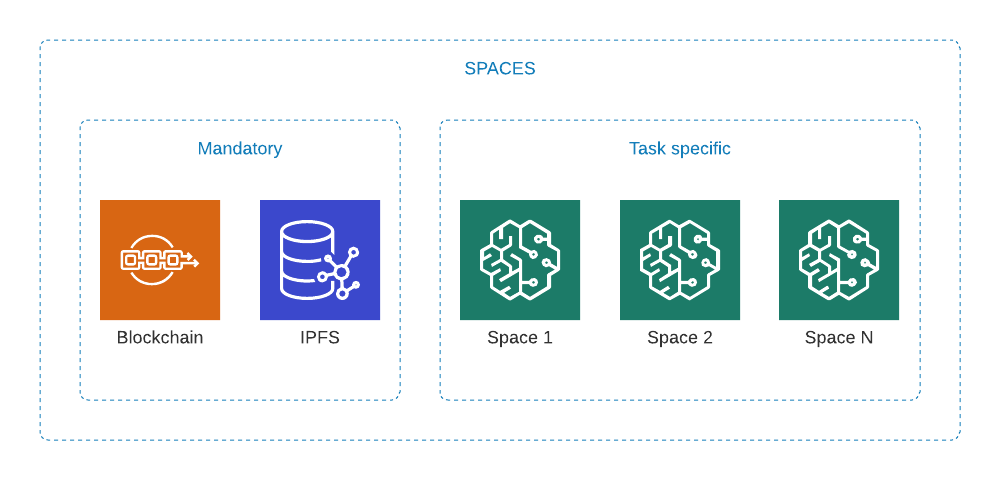
\includegraphics[width=10cm]{spaces}
\caption{Spaces}
\end{figure}

Mandatory \textbf{spaces} are always up and performs network maintainance and support functions.
Task specific \textbf{spaces} running on-demand and depends of type of task which needs to be done.

System data collected by \textbf{ORC}:

\begin{itemize}
    \item CPU information eg. amount, speed and utilization of cores
    \item GPU information including amount and model of GPUs, memory size and amount of graphic processors
    \item Total and free disk space, IO metrics
    \item Total and free memory amount
    \item Performance metrics like request-response time, network latency and so on
\end{itemize}

These data is used to improve the quality of nodes and exclude low performance nodes or non stable ones.

For cases when it's impossible to use IPFS for task data \textbf{ORC} will use internal storage.

\section{Tasks}

Task is a set of actions which should be performed on the node.
Also task must contain the list of system requirements which is necessary for its execution.

To describe the task the following type specification must be used:

\begin{minted}{erlang}
-type xpu() :: <<"cpu">> | <<"nvidia">> | <<"amd">>.

-type step() :: #{
    <<"name">>    => binary(),
    step_module() := step_args()
}.

-type task() :: #{
    <<"name">>                   => binary(),
    <<"xpu">>                    := xpu(),
    <<"xpu-cpu-fallback">>       := boolean(),
    <<"xpu-n">>                  := pos_integer(),
    <<"xpu-fallback-wait-time">> => pos_integer(),
    <<"pending-ttl">>            => pos_integer(),
    <<"ttl">>                    => pos_integer(),
    <<"spaces">> := #{
        xpu() := binary()
    },
    <<"steps">> := [step()]
}.
\end{minted}

\begin{itemize}
    \item name - human readable description of the task
    \item xpu - the type of execution unit, can be \textbf{cpu}, \textbf{nvidia} or \textbf{amd} if task require GPU
    \item xpu-cpu-fallback - in case if xpu is set to use GPU but no node with GPU found during \textbf{xpu-fallback-wait-time} time task will assigned to node with CPU only
    \item xpu-n - minimum amount of the required execution units eg. amount of GPUs or CPU cores
    \item pending-ttl - task will be canceled if no one node will found during \textbf{pending-ttl} period
    \item ttl - maximum task execution time
    \item spaces - the list of specific isolated environments per xpu type
    \item steps - the list of actions which should be performed on the node
\end{itemize}

More detailed specification may be found in the project OSS\cite{oss} documents.

Task can be described using both JSON or YAML formats.

\newpage
Neural Style Transfer task example described in JSON:

\inputminted{json}{neural-style-task.json}

\newpage
GPU mining task example described in YAML format:

\inputminted{yaml}{claymore-cuda-mining-task.yaml}

\section{Reputation}

Reputation is an entity which consists of several values and represents the quality of the user's nodes.
It also helps to detect the non stable or malicious nodes,
increases the efficiency of the node selection algorithm and
affects the total reward amount.

Reputation is calculating on the daily basis consists of the following parameters:

\begin{itemize}
    \item Uptime (U) - the mean value of the nodes uptime
    \item Completed tasks (C) - the percentage of completed tasks
\end{itemize}

More parameters may be added if necessary.

The common reputation formula looks like:

\[
    R = \frac{\sum(U, C, ...)}{\vert{N}\vert}
\]

Where \textbf{N} is amount if items used in calculation.
The final value of the reputation is calculated for the 30 days period.

\subsection{Uptime}

Uptime is the measure of the uninterrupted time that a node system experiences.

We use the mean value of the uptime - sum of uptime of all users nodes divided by nodes amount.

\[
    U = \frac{\sum(u) / 2592000}{N}
\]

Where \textbf{u} is an uptime of the specific node, \textbf{2592000} is amount of seconds in 30 days and \textbf{N} is the total amount of nodes which are in online state.

\subsection{Completed tasks}

\[
    C = \frac{C}{N / 100}
\]

Where \textbf{C} is an amount of the completed tasks and \textbf{N} is the total amount of tasks accepted by the user's nodes.

\subsection{Examples}

User has 3 nodes - node A, node B and node C. During the last 30 days these nodes were online the following amount of seconds:

\begin{itemize}
    \item A - 2246400 seconds, 4 days downtime
    \item B - 1987200 seconds, 7 days downtime
    \item C - 2505600 seconds, 1 day downtime
\end{itemize}

According the to values above the mean uptime will be:

\[
    U = \frac{(2246400 + 1987200 + 2505600) / 2592000}{3} = 0.86 * 100 = 86\%
\]

Also these nodes accepted 743 tasks and 345 tasks were succesful, others one are canceled or failed or expired.

So to calculate the percent of completed task we apply the following formula:

\[
    C = \frac{345}{743 / 100} = 46.43\%
\]

The final reputation value will be:

\[
    R = \frac{86 + 46.43}{2} = 66.21\%
\]

\section{Blockchain}

The Aeternity technologies are used as blockchain backbone for the project.
It was chosen because of the rich features like oracles, state channels and so on.

The project uses dedicated chain.
Initially it's a plan to utilize the blockchain only as a payment system.
But in the future all the things like tasks management, rewards, etc will be implemented as smart contracts.


\bibliography{paper}
\bibliographystyle{plain}

\end{document}
